\chapter{Results}\label{sec:results}
We now describe the results of testing the ILP systems. Due to restraints on computational power we tested the performance of the each ILP on 8 full game play outs. 15 minutes were given for each system to generate a hypothesis. We trained the systems on random gameplay, gameplay generated by the Sancho system and then a mixture of both. The generated hypotheses were tested on both Sancho generated and random gameplay examples.



Q1 Does varying the quality of game traces influence the ability for learners to solve the IGGP problems? Specifically, does the quality of game play affect predictive accuracy?
Q2 Does varying the amount of game traces influence the ability for learners to solve the IGGP problems? Specifically, does the quality of game play affect predictive accuracy?
Q3 Can we improve the performance of a learner by mixing the quality of traces?

\section{Evaluation metrics}
To evaluate the performance of the ILP systems on the training dataset we use two metrics: balanced accuracy and perfectly solved.

\textbf{Balanced accuracy} In the datasets used for testing the ILP systems the vast majority of examples are negative. Balanced accuracy takes this into account when evaluating approaches. The system to be tested is the generated logical hypothesis $H$ which, along with the background knowledge $B$ for the relevant game. The test data is the set of combined positive and negative testing examples $E^+ \cup E^-$. We define the number of positive examples $p = |E^+|$, the number of negative examples $n = |E^-|$, the number of correctly predicted positives as $tp = |\{e\in E^+|B\cup H \models e\}|$ and the number of correctly predicted negatives as $tn = |\{e\in E^-|B\cup H \not\models e\}|$. The balanced accuracy is subsequently defined as $ba = 100 \cdot (tp/p + tn/n)/2$.

\textbf{Perfectly solved} This metric considers the number of predicates for which the ILP system correctly classified all examples. It is equivalent to the number of games with a balanced accuracy score of 100. This metric is important since for all predicates there exists an exact solution (the rules that were used to generate the examples). A system that has correctly predicated 99\% of the results is no where near as useful as one that predicts 100\%.

\section{Answering research questions}
To answer the research questions one and three we train the three ILP systems on random, Sancho generated game traces as well as a mixture of the two. We compare the average balanced accuracy and the number of perfectly solved games of the different systems trained on the range of domains. 

To answer question two we train the systems on the mixed traces with varying size of data to see how it affects the test results. We train on the mixed traces since this gave the best results in the first set of experiments.
\section{Results summary}
We found that 
\section{Varying quality training data}

\subsubsection{Random training}
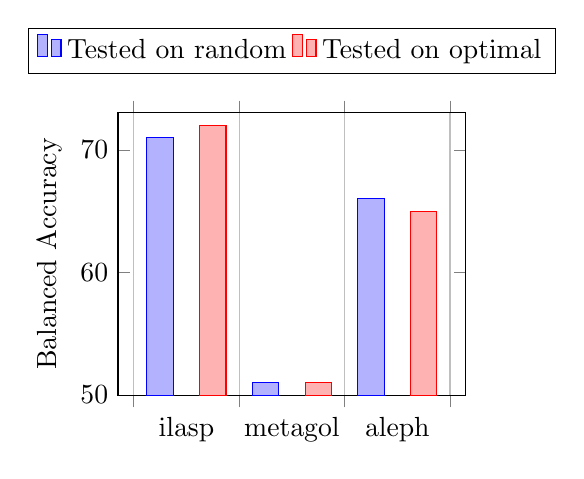
\begin{tikzpicture}
\begin{axis}[
	ylabel=Balanced Accuracy,
	width=6cm,
	enlargelimits=0.05,
	legend style={at={(0.5,1.3)},
	anchor=north,
	legend columns=-1},
	ybar interval=0.5,
	symbolic x coords={ilasp,metagol,aleph, poog}
]
\addplot 
	coordinates {(ilasp,71) (metagol,51) (aleph,66) (poog, 65)};
\addplot 
	coordinates {(ilasp,72) (metagol,51) (aleph,65) (poog,65)};
\legend{Tested on random,Tested on optimal}
\end{axis}
\end{tikzpicture}
~
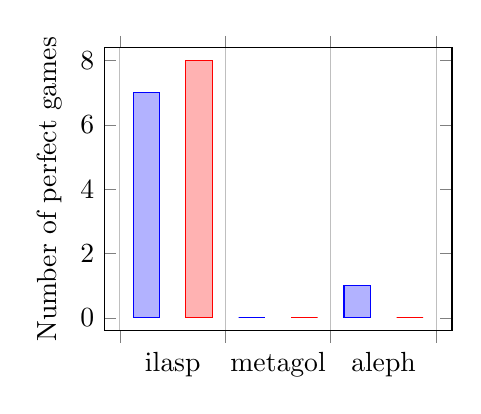
\begin{tikzpicture}
\begin{axis}[
	width=6cm, 
	ylabel=Number of perfect games,
	enlargelimits=0.05,
	ybar interval=0.5,
	symbolic x coords={ilasp,metagol,aleph, poog}
]
\addplot 
	coordinates {(ilasp,7) (metagol,0) (aleph,1) (poog, 0)};
\addplot 
	coordinates {(ilasp,8) (metagol,0) (aleph,0) (poog,0)};
\end{axis}
\end{tikzpicture}
\subsubsection{Optimal training}
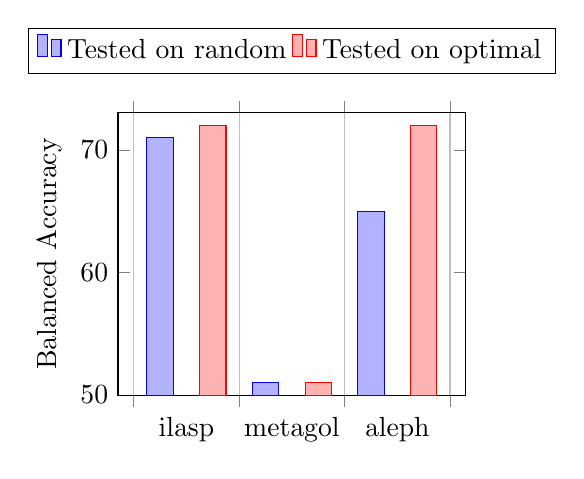
\begin{tikzpicture}
\begin{axis}[
ylabel=Balanced Accuracy,
width=6cm,
enlargelimits=0.05,
legend style={at={(0.5,1.3)},
	anchor=north,
	legend columns=-1},
ybar interval=0.5,
symbolic x coords={ilasp,metagol,aleph, poog}
]
\addplot 
coordinates {(ilasp,71) (metagol,51) (aleph,65) (poog, 65)};
\addplot 
coordinates {(ilasp,72) (metagol,51) (aleph,72) (poog,65)};
\legend{Tested on random,Tested on optimal}
\end{axis}
\end{tikzpicture}
~
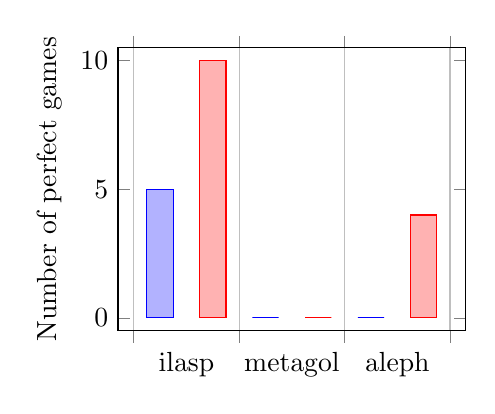
\begin{tikzpicture}
\begin{axis}[
width=6cm, 
ylabel=Number of perfect games,
enlargelimits=0.05,
ybar interval=0.5,
symbolic x coords={ilasp,metagol,aleph, poog}
]
\addplot 
coordinates {(ilasp,5) (metagol,0) (aleph,0) (poog, 0)};
\addplot 
coordinates {(ilasp,10) (metagol,0) (aleph,4) (poog,0)};
\end{axis}
\end{tikzpicture}
\subsubsection{Mixed training}
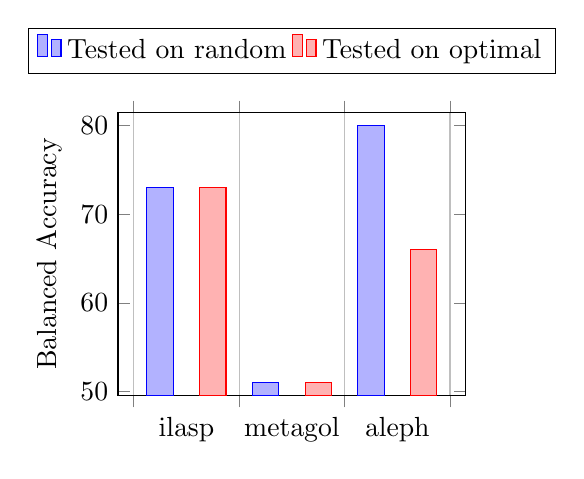
\begin{tikzpicture}
\begin{axis}[
ylabel=Balanced Accuracy,
width=6cm,
enlargelimits=0.05,
legend style={at={(0.5,1.3)},
	anchor=north,
	legend columns=-1},
ybar interval=0.5,
symbolic x coords={ilasp,metagol,aleph, poog}
]
\addplot 
coordinates {(ilasp,73) (metagol,51) (aleph,80) (poog,70)};
\addplot 
coordinates {(ilasp,73) (metagol,51) (aleph,66) (poog,70)};
\legend{Tested on random,Tested on optimal}
\end{axis}
\end{tikzpicture}
~
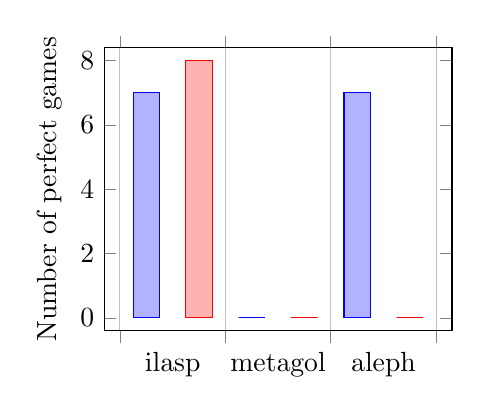
\begin{tikzpicture}
\begin{axis}[
width=6cm, 
ylabel=Number of perfect games,
enlargelimits=0.05,
ybar interval=0.5,
symbolic x coords={ilasp,metagol,aleph, poog}
]
\addplot 
coordinates {(ilasp,7) (metagol,0) (aleph,7) (poog, 0)};
\addplot 
coordinates {(ilasp,8) (metagol,0) (aleph,0) (poog,0)};
\end{axis}
\end{tikzpicture}

\subsubsection{Mixed training with 16 traces}
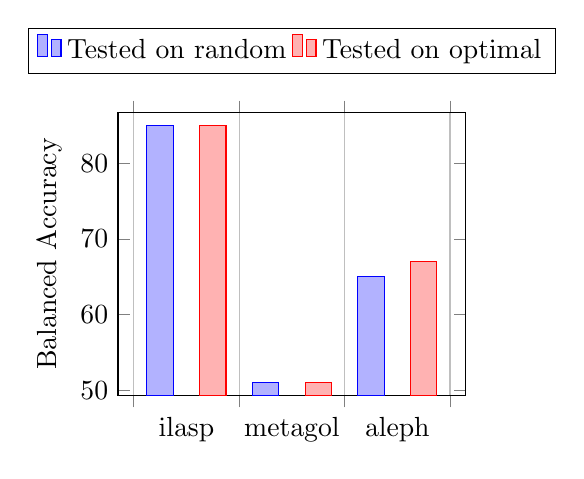
\begin{tikzpicture}
\begin{axis}[
ylabel=Balanced Accuracy,
width=6cm,
enlargelimits=0.05,
legend style={at={(0.5,1.3)},
	anchor=north,
	legend columns=-1},
ybar interval=0.5,
symbolic x coords={ilasp,metagol,aleph, poog}
]
\addplot 
coordinates {(ilasp,85) (metagol,51) (aleph,65) (poog,70)};
\addplot 
coordinates {(ilasp,85) (metagol,51) (aleph,67) (poog,70)};
\legend{Tested on random,Tested on optimal}
\end{axis}
\end{tikzpicture}
~
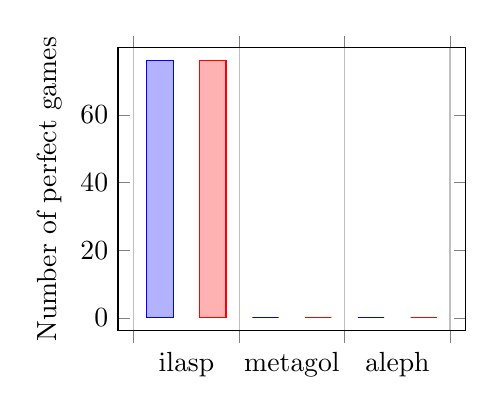
\begin{tikzpicture}
\begin{axis}[
width=6cm, 
ylabel=Number of perfect games,
enlargelimits=0.05,
ybar interval=0.5,
symbolic x coords={ilasp,metagol,aleph, poog}
]
\addplot 
coordinates {(ilasp,76) (metagol,0) (aleph,0) (poog, 0)};
\addplot 
coordinates {(ilasp,76) (metagol,0) (aleph,0) (poog,0)};
\end{axis}
\end{tikzpicture}

\subsubsection{Mixed training with 24 traces}
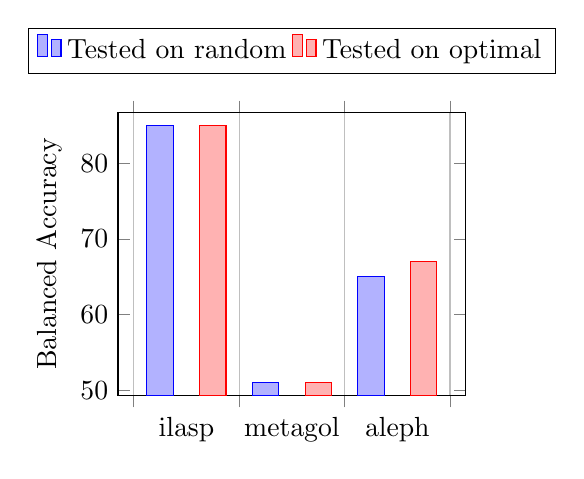
\begin{tikzpicture}
\begin{axis}[
ylabel=Balanced Accuracy,
width=6cm,
enlargelimits=0.05,
legend style={at={(0.5,1.3)},
	anchor=north,
	legend columns=-1},
ybar interval=0.5,
symbolic x coords={ilasp,metagol,aleph, poog}
]
\addplot 
coordinates {(ilasp,85) (metagol,51) (aleph,65) (poog,70)};
\addplot 
coordinates {(ilasp,85) (metagol,51) (aleph,67) (poog,70)};
\legend{Tested on random,Tested on optimal}
\end{axis}
\end{tikzpicture}
~
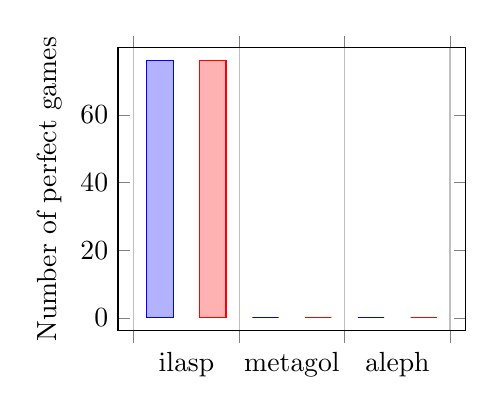
\begin{tikzpicture}
\begin{axis}[
width=6cm, 
ylabel=Number of perfect games,
enlargelimits=0.05,
ybar interval=0.5,
symbolic x coords={ilasp,metagol,aleph, poog}
]
\addplot 
coordinates {(ilasp,76) (metagol,0) (aleph,0) (poog, 0)};
\addplot 
coordinates {(ilasp,76) (metagol,0) (aleph,0) (poog,0)};
\end{axis}
\end{tikzpicture}

